\documentclass[utf8x]{beamer}

\usepackage{beamerthemesplit}
\usepackage{url}
\usepackage{amsmath}
\usepackage{amssymb}
\usepackage{verbatim}
\usepackage{hyperref}
\usepackage{pgf,tikz}
\usetikzlibrary{arrows}


\makeatletter
\AtBeginDocument{% example environment modified from the example environment in lshort.sty, using the verbatim package
  \newwrite\examplesx@out
  \newenvironment{examplesx}{%
    \begingroup% Lets Keep the Changes Local
      \@bsphack
      \immediate\openout \examplesx@out \jobname.exa
      \let\do\@makeother\dospecials\catcode`\^^M\active
      \def\verbatim@processline{%
        \immediate\write\examplesx@out{\the\verbatim@line}}%
      \verbatim@start
    }{%
    \immediate\closeout\examplesx@out\@esphack\endgroup%
    \noindent\makebox[\textwidth][l]{%
      \begin{minipage}[c]{0.45\textwidth}%
        \small\verbatiminput{\jobname.exa}
      \end{minipage}%
      \hspace*{0.1\textwidth}%
      \framebox{%
        \begin{minipage}{0.45\textwidth}%
          \small\input{\jobname.exa}%
        \end{minipage}
      }%
    }\vspace*{\parskip}%
  }
}
\makeatother

\pdfinfo {
  /Title (Cluedump -- LaTeX)
  /Subject (LaTeX)
  /Author (Jason Gross)
  /Keywords (Cluedump, SIBP, LaTeX)
}

\begin{document}

\title{Cluedump -- \LaTeX}
\date{November 2, 2010}
\author{Jason Gross --- \href{mailto:jgross@mit.edu}{jgross@mit.edu}}

\begin{frame}
  \titlepage
  This document is available at \url{http://web.mit.edu/jgross/Public/2010cluedump/\jobname.pdf}.
\end{frame}

\section*{Outline}
  \begin{frame}
    \frametitle{Outline}
    \tableofcontents[pausesections]
  \end{frame}
\section{Getting Started}
  \subsection{Installing \LaTeX}
    \begin{frame}
      \frametitle{\LaTeX{} on Linux}
      \begin{itemize}
        \item Usually comes preinstalled
        \item \TeX Live can be downloaded from \url{http://www.tug.org/texlive/}
        \item Use your favorite text editor (vim, emacs, etc.), OR
        \item Specialized editors for \LaTeX, e.g. kile (\url{http://kile.sourceforge.net/})
          \begin{itemize}
            \item \texttt{sudo apt-get install kile okular}
          \end{itemize}
      \end{itemize}
  %       \begin{center}
  %         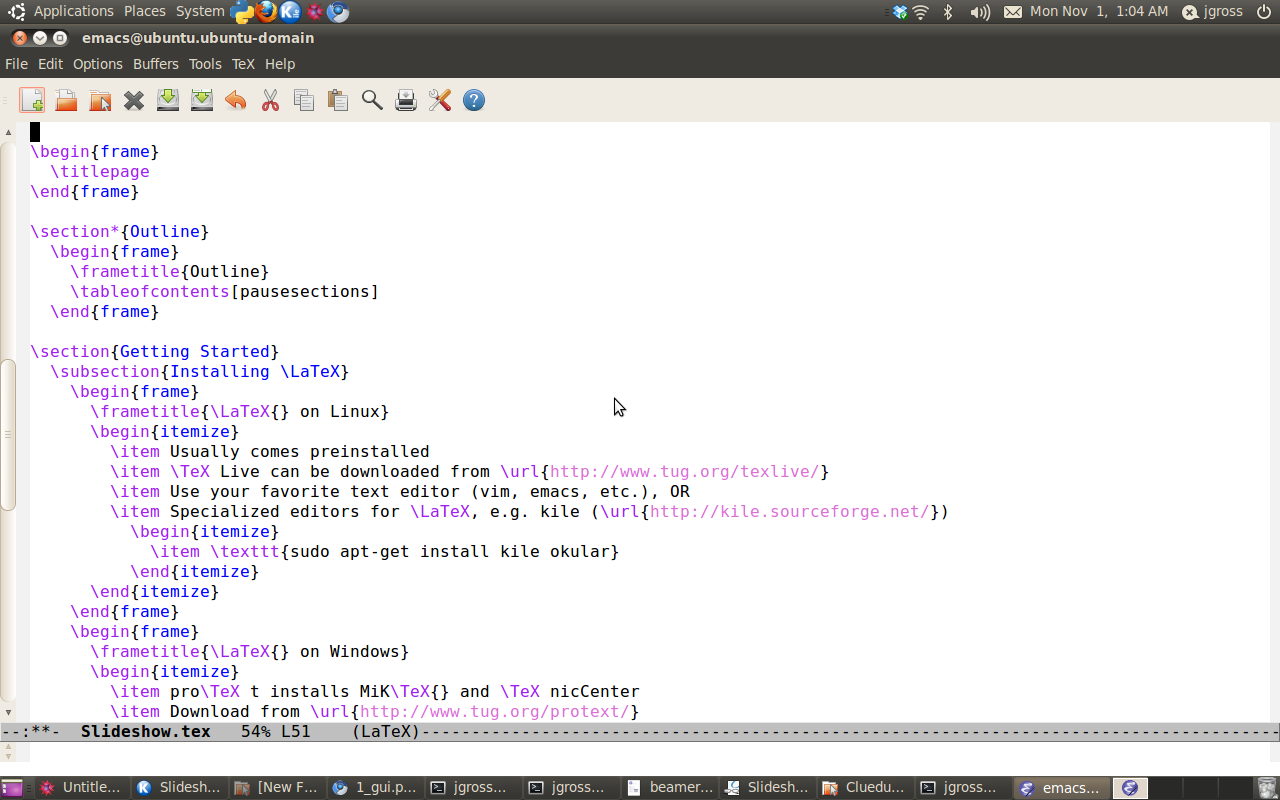
\includegraphics[width=0.2\textwidth]{emacs}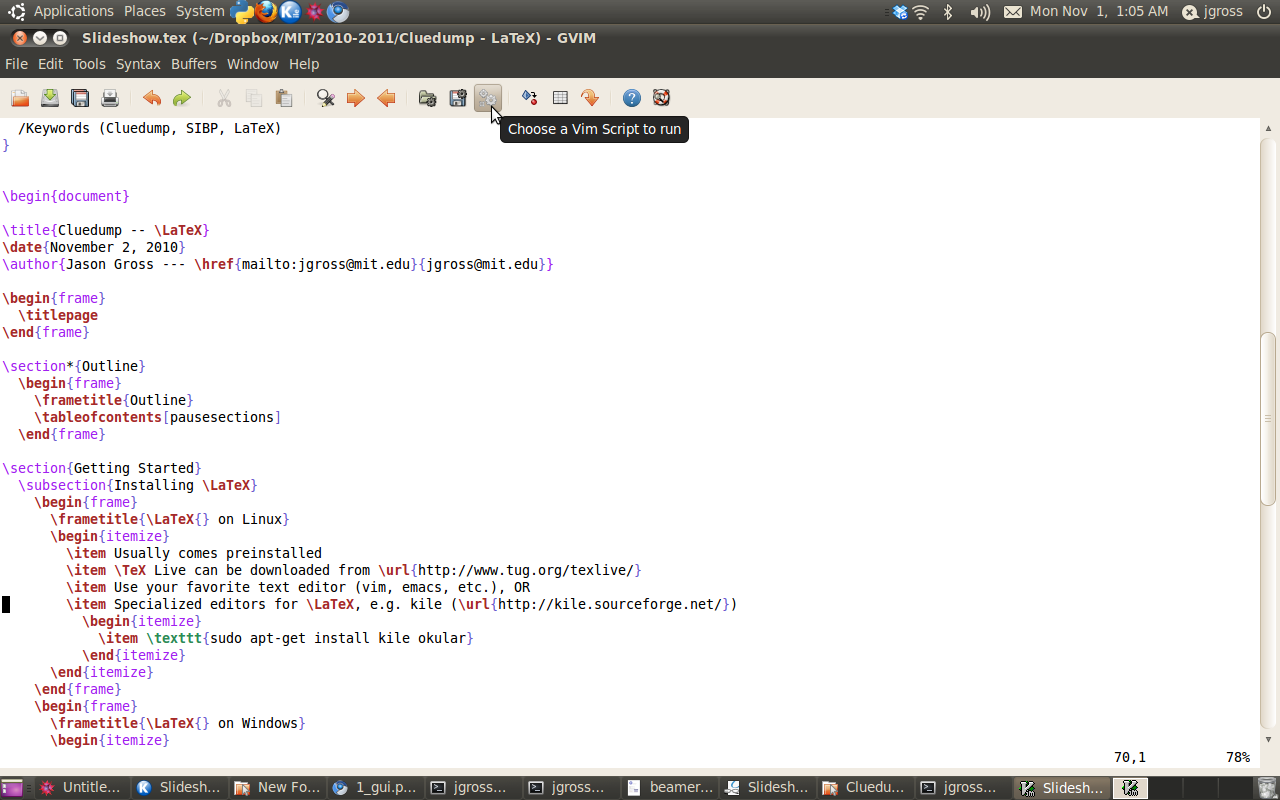
\includegraphics[width=0.2\textwidth]{gvim}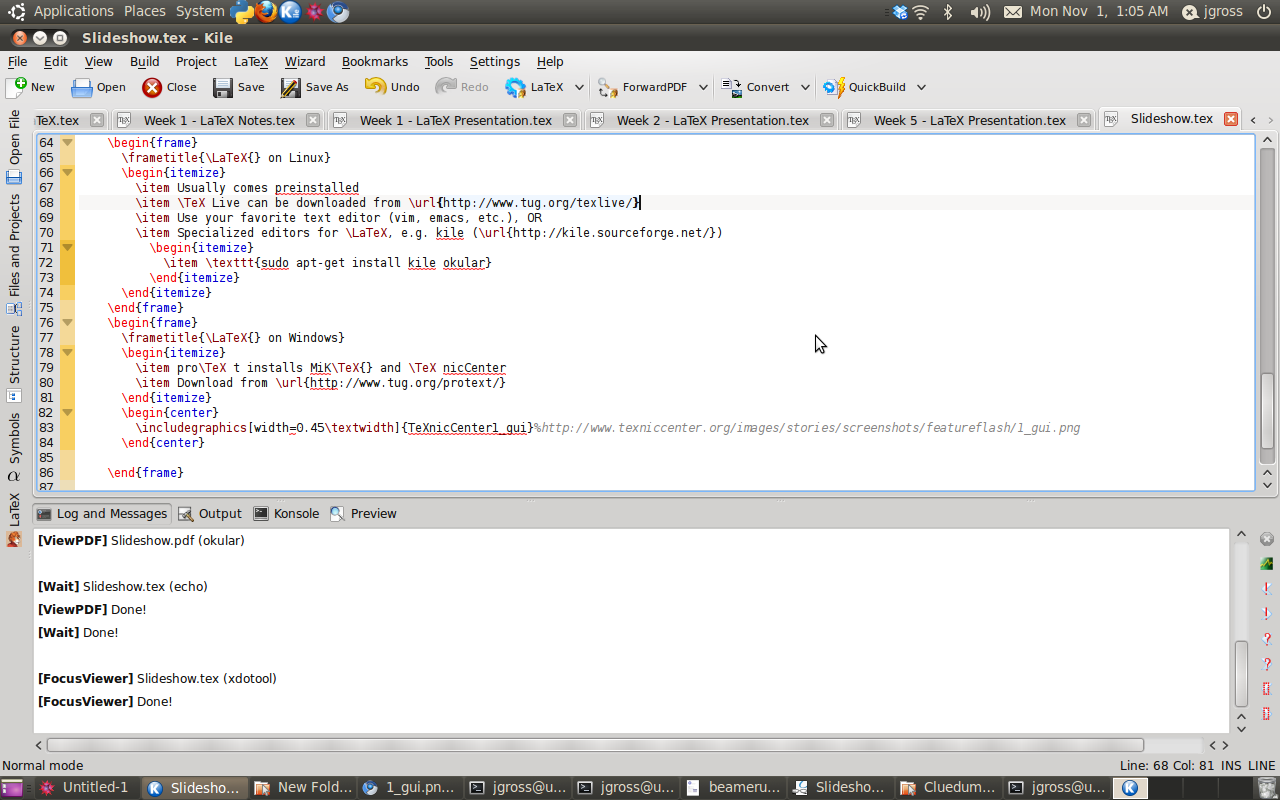
\includegraphics[width=0.2\textwidth]{kile}
  %       \end{center}
    \end{frame}
    \begin{frame}
      \frametitle{\LaTeX{} on Windows}
      \begin{itemize}
        \item pro\TeX t installs MiK\TeX{} and \TeX nicCenter
        \item Download from \url{http://www.tug.org/protext/}
      \end{itemize}
      \begin{center}
        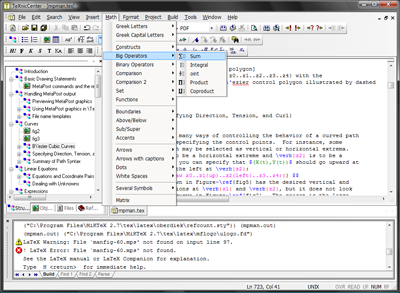
\includegraphics[width=0.45\textwidth]{TeXnicCenter1_gui}%http://www.texniccenter.org/images/stories/screenshots/featureflash/1_gui.png
      \end{center}
    \end{frame}
    \begin{frame}
      \frametitle{\LaTeX{} on Mac}
      \begin{itemize}
        \item Mac\TeX{} (\url{http://www.tug.org/mactex/})
        \item \TeX Shop (\url{http://pages.uoregon.edu/koch/texshop/})
      \end{itemize}
      \begin{center}
        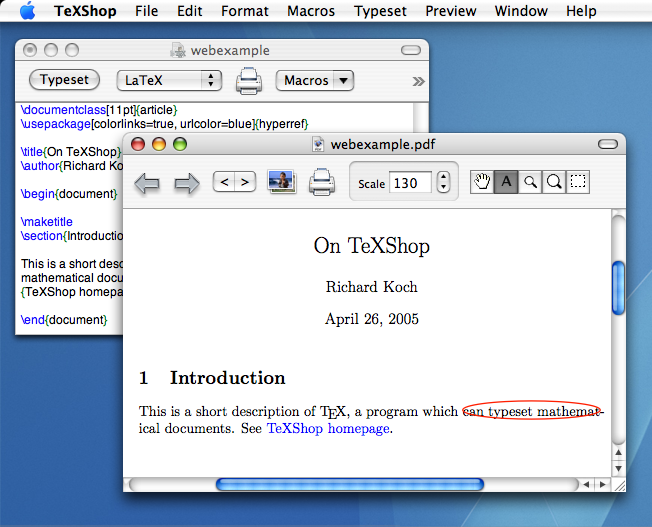
\includegraphics[width=0.45\textwidth]{TeXshop}%http://pages.uoregon.edu/koch/texshop/
      \end{center}
    \end{frame}

  \subsection{What is \LaTeX?}
    \begin{frame}
      \frametitle{What \LaTeX{} is}
      \begin{itemize}
        \item A typesetting system \pause
        \item Aimed at math and text \pause
        \item Extensible \pause
        \item A macro-based Turing complete programming language
      \end{itemize}
    \end{frame}
    \begin{frame}
      \frametitle{What \LaTeX{} is not}
      \begin{itemize}
        \item A WYSIWYG editor
        \begin{center}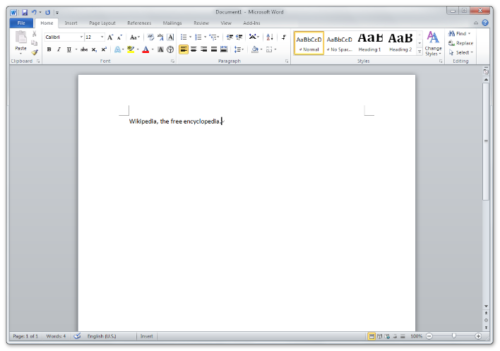
\includegraphics[width=0.3\textwidth]{Word_2010}\end{center}% http://upload.wikimedia.org/wikipedia/en/2/2a/Word_2010.png
        \pause \item A programming language
        \begin{center}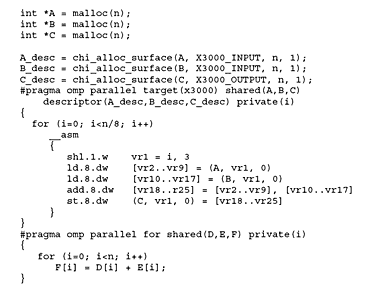
\includegraphics[width=0.3\textwidth]{programming}\end{center}%http://www.intel.com/technology/itj/2007/v11i3/2-exoskeleton/5-environment.htm
      \end{itemize}
    \end{frame}
  \subsection{Getting Help}
    \begin{frame}[containsverbatim]
      \frametitle{Finding Help}
      \begin{itemize}
        \item lshort: This is the biggest beginner help file available on the web for \LaTeX{}. Go to \url{http://mirror.ctan.org/info/lshort/english/lshort.pdf}. Alternatively, Google \textit{lshort} and it will come up.
        \item Google: One of the best help files out there. Google anything you want to accomplish along with \LaTeX{} and you will get something. Unless of course you type \verb|"Build a time machine" latex|.
        \item \url{http://www.ctan.org}: Gives the full documentation for any package, the source code, etc.
        \item \url{http://detexify.kirelabs.org/classify.html}. Slightly more useful for tablets, but useful nonetheless.
      \end{itemize}
    \end{frame}

  \subsection{Basic Setup}
    \begin{frame}[containsverbatim]
      \frametitle{Document Structure}
      \noindent \verb|\documentclass{|\emph{document class}\verb|}| \\
      \noindent \emph{preamble} \\
      \noindent \verb|\begin{document}| \\
      \noindent \emph{document body} \\
      \noindent \verb|\end{document}|
    \end{frame}
    \begin{frame}[containsverbatim]
      \frametitle{Document Structure}
      \begin{verbatim}
        \documentclass{article}
        \usepackage{amsmath}
        \begin{document}
          Your stuff goes here!
        \end{document}
      \end{verbatim}
    \end{frame}
    \begin{frame}[containsverbatim]
      The default given is the \verb|article| document type, but there are others available: \verb|report|, \verb|book|, \verb|letter|, \verb|slides|. You can also set options for your document: \verb|\documentclass[11pt, letterpaper, landscape, twoside]|\\ \verb|{article}|. Refer to the help files for more details.
    \end{frame}
\section{Basic Typesetting}
  \subsection{Good Practices}
    \begin{frame}[containsverbatim,allowframebreaks]
      \frametitle{Guiding Principles}
      \begin{itemize}
        \item You're not a professional typesetter!  Don't override \LaTeX's default formatting (including font sizes) unless you have a \emph{very} good reason for doing so.
        \item The default margins are large. It is easier to read papers if there are no more than $80$ characters on a line; this is why newspapers have multiple columns.
        \item \LaTeX{} (mostly) ignores duplicated white space. If you have two or more returns in a row, this makes a new line. Don't tell \LaTeX{} to make multiple blank lines because it knows how to make things more readable. The one major exception to this rule is math mode. \pause
        \item Every so often in the source code press enter (to make it readable - about every $80$ characters). This won't affect your output because \LaTeX{} doesn't render single line breaks.
        \item Use logical structure in your documents. Don't hardcode (too much) formatting into your document; use predefined \LaTeX{} commands (like \verb|\subsection{}|, etc.).
        \item (For advanced \LaTeX{} users) Don't define too many macros, use obscure packages not on CTAN, and do other weird things like that. If you do, publishers won't like you very much.
      \end{itemize}
    \end{frame}
  \subsection{Optional (but useful) packages}
    \begin{frame}[containsverbatim]
      \frametitle{Optional (but useful) packages}
      Packages provided added functionality for your \LaTeX{} code. To include a package use the command \verb|\usepackage[|\textit{(optional) Options}\verb|]{|\textit{Package name}\verb|}|.
      \begin{table}[h]
        \begin{tabular}{c|p{6cm}}
          Package name & Description\\\hline
          \verb|amsmath| & Gives an environment for typsetting math formulas. Namely\newline \verb|\begin{equation}|\newline \verb|\end{equation}|, among other things.\\
          \verb|amssymb| & Gives mathematical symbols that may not be built into \LaTeX{}\\
          \verb|amsthm| & Gives an environment for typing theorems in a standard format\\
        \end{tabular}
      \end{table}
    \end{frame}
    \begin{frame}[containsverbatim]
      \frametitle{Optional (but useful) packages}
      \begin{table}[h]
        \begin{tabular}{c|p{6cm}}
          Package name & Description\\\hline
          \verb|graphicx| & Can insert pictures from .jpg, .pdf, .png, .eps, among others using the \verb|\includegraphics[|\textit{(optional) Options}\verb|]{|\textit{filename}\verb|}|\\
          \verb|hyperref| & Lets you make hyperlinks\\
          \verb|geometry| & Lets you change the margins\\
          \verb|enumerate| & Lets you control the \verb|enumerate| environment for lists and outlines\\
        \end{tabular}
      \end{table}
      You'll want to load \verb|amsmath| and \verb|amssymb| for any sort of math typsetting.
    \end{frame}

  \subsection{\LaTeX{} and Math}
    \subsection{Basic math typsetting}
      \subsubsection{Ways to get into math mode}
        \begin{frame}[containsverbatim]
          \frametitle{Ways to get into math mode}
          \begin{itemize}
            \item As you are typing regular text, put any math mode commands (or math) between \$\$ like so: \verb|$\frac{3}{4}$| (this will look like $\frac{3}{4}$). This can be inserted right in the middle of text: \verb|The answer is $x = 3$.|
            \item Use the package \verb|amsmath| and then use \verb|\begin{equation}\end{equation}| (numbers your lines between the two commands) or \verb|\begin{equation*}\end{equation*}| (does not number your lines).
            \item Place math between \verb|\[|\textit{insert math here}\verb|\]| or \verb|$$|\textit{insert math here}\verb|$$| to get it centered on a new line.
          \end{itemize}
        \end{frame}
      \subsubsection{A few common math things}
      \makeatletter
      \newcommand{\myverb}[1]{{\@vobeyspaces\obeyspaces\frenchspacing\texttt{\detokenize{#1}}}}
        \begin{frame}
          \frametitle{A few common math things}
          A more exhaustive list can be found through the lshort reference.
          \begin{itemize}
            \item Fractions: \myverb{$\frac{1}{4}$} ($\frac{1}{4}$), \myverb{$\frac{1 + \frac{1}{3}}{2x + \frac{1}{5}}$} ($\frac{1 + \frac{1}{3}}{2x + \frac{1}{5}}$)
            \pause \item Exponents and subscripts: \myverb{$x_1^2 + x_2^2 + \cdots + x_{11}^2$} ($x_1^2 + x_2^2 + \cdots + x_{11}^2$), \myverb{$(3x + 7)^{100}$} ($(3x + 7)^{100}$)
            \pause \item Trig functions: \myverb{$\cos(\sin x)$} ($\cos(\sin x)$)
            \pause \item Summations: \myverb{$\sum_{i = 0}^5 (ar^n)$} ($\sum_{i = 0}^5 (ar^n)$)
            \pause \item Integrals: \myverb{$\int_0^{\pi/2}e^x \ln x\,dx$} ($\int_0^{\pi/2}e^x \ln x\,dx$)
            \pause \item Square roots and \emph{n}$^\text{th}$ roots: \myverb{$\sqrt{x^2 + 1}$} ($\sqrt{x^2 + 1}$), \myverb{$\sqrt[3]{8} = 2$} ($\sqrt[3]{8} = 2$)
            \pause \item Greek letters: \myverb{$\pi$} ($\pi$), \myverb{$\Omega$} ($\Omega$), \myverb{$\omega$} ($\omega$)
          \end{itemize}
        \end{frame}

      \subsubsection{A few not so common math things}
        \begin{frame}[containsverbatim]
          \frametitle{A few not so common math things}
          \begin{itemize}
            \item Spaces in math mode are tricky. Here are some ways to fix up spaces:
            \begin{center}
              \begin{tabular}{l|l|l}
                Symbol & Code & Example \\ \hline
                \verb|\!| & \verb|x \! y| & $x \! y$ \\
                \verb|\,| & \verb|x \, y| & $x \, y$ \\
                \verb|\:| & \verb|x \: y| & $x \: y$ \\
                \verb|\;| & \verb|x \; y| & $x \; y$ \\
                \verb|\ | & \verb|x \  y| & $x \ y$ \\
                \verb|\quad| & \verb|x \quad y| & $x \quad y$ \\
                \verb|\qquad| & \verb|x \qquad y| & $x \qquad y$ \\

              \end{tabular}
            \end{center}
            \item How to box an answer (only in text mode):
              \verb|\framebox[|\textit{width}\verb|][|\textit{position (l, c, r)}\verb|]{|\textit{text}\verb|}|

              For example, Einstein said, \framebox{$E = mc^2$}!
          \end{itemize}
        \end{frame}
\section{Miscellaneous}
  \subsection{Things to watch out for}
    \begin{frame}[containsverbatim]
      \frametitle{Just a few reminders/cautions:}
      \begin{itemize}
        \item \LaTeX{} is case-sensitive (for the most part), so if you are getting strange compiler errors, check your capitalization.
        \item Some characters are only available in math mode (e.g. $<$, $>$)
        \item Special characters that \LaTeX{} will get angry about:
        \verb|#|, \verb|$|, \verb|%|, \verb|^|, \verb|&|, \verb|_|, \verb|{|, \verb|}|, \verb|~|, \verb|\|. To typeset these, use this instead: \verb|\#|, \verb|\$|, \verb|\%|, \verb|\^{}|, \verb|\&|, \verb|\_|, \verb|\{|, \verb|\}|, \verb|\~{}|, \verb|\textbackslash|
      \end{itemize}
    \end{frame}

  \subsection{Other environments}
    \begin{itemize}
    \begin{frame}[containsverbatim]
      \frametitle{The list environment}
      \item Lists: Here are two examples of lists and their output: \par $\left.\right.$ \par

\begin{examplesx}
\begin{itemize}
  \item Math
  \item Chemistry
  \item Physics
\end{itemize}
\end{examplesx}
    \end{frame}
    \begin{frame}[containsverbatim]
      \frametitle{Another list environment}
\begin{examplesx}
\begin{enumerate}
    \item Math
    \item Chemistry
    \item Physics
\end{enumerate}
\end{examplesx}
    \end{frame}
    \begin{frame}[containsverbatim]
      \frametitle{The tabular environment}
      \item Tables:  \par $\left.\right.$ \par

\begin{examplesx}
\begin{tabular}{l|cc}
    Number & Numeral & Roman
    \\ \hline
    Five & $5$ & $V$\\
    Ten & $10$ & $X$\\
\end{tabular}
\end{examplesx}
    \end{frame}

    \begin{frame}[containsverbatim]
      \frametitle{Aligned equations}
      \item Aligned equations: \\

\begin{examplesx}
\begin{align}
  f(x) & = 9y^2 - 6y \nonumber\\
       & = (9y^2 - 6y + 1) - 1
          \nonumber \\
       & = (3y - 1)^2 - 1
\end{align}
\end{examplesx}
    \end{frame}

    \begin{frame}[containsverbatim]
      \frametitle{The \texttt{section} command}
      \item Sections: \\
\begin{verbatim}
\section{Scientists}
  \subsection{Euler}
    He knew everything.
  \subsection{Newton}
    He knew gravity.
\section{Students}
  \section{MIT Students}
    \subsubsection*{Jason}
      He knows \LaTeX.
    \subsubsection*{Piper}
      She's running cluedumps.
\end{verbatim}
        \qquad \begin{pgfpicture}{-6.4cm}{0cm}{4cm}{-6cm}
        \pgfdeclareimage[height=6cm]{img}{Sections-crop}
        \pgfuseimage{img}
      \end{pgfpicture}
    \end{frame}
  \end{itemize}

\section{Graphics}
  \subsection{Basics}
    \begin{frame}[containsverbatim]
      \frametitle{graphicx}
      The simplest way is to \verb|\usepackage{graphicx}| and then \verb|\includegraphics{|\emph{file name}\verb|}|.

      For example,
\begin{verbatim}
\begin{center}

\includegraphics[height=0.5\textheight]{grumpyfuzzball}
\end{center}
\end{verbatim}
      gives me
      \begin{center}
\includegraphics[height=0.5\textheight]{grumpyfuzzball}\end{center}
    \end{frame}
  \subsection{Intermediate}
    \begin{frame}[containsverbatim]
      \frametitle{Picture}
\begin{examplesx}
\setlength{\unitlength}{0.8cm}
\begin{picture}(6,5)
\thicklines
\put(1,0.5){\line(2,1){3}}
\put(4,2){\line(-2,1){2}}
\put(2,3){\line(-2,-5){1}}
\put(0.7,0.3){$A$}
\put(4.05,1.9){$B$}
\put(1.7,2.95){$C$}
\put(3.1,2.5){$a$}
\put(1.3,1.7){$b$}
\put(2.5,1.05){$c$}
\put(0.3,4){$F=
\sqrt{s(s-a)(s-b)(s-c)}$}
\put(3.5,0.4){$\displaystyle s:=\frac{a+b+c}{2}$}
\end{picture}
\end{examplesx}
   \end{frame}
  \subsection{Advanced}
    \begin{frame}[containsverbatim]
      \frametitle{pgf/tikz}
\begin{examplesx}
\begin{tikzpicture}[scale=2]
\clip (-0.1,-0.2)
rectangle (1.8,1.2);
\draw[step=.25cm,gray,very thin]
(-1.4,-1.4) grid (3.4,3.4);
\draw (-1.5,0) -- (2.5,0);
\draw (0,-1.5) -- (0,1.5);
\draw (0,0) circle (1cm);
\filldraw[fill=green!20!white,
draw=green!50!black]
(0,0) -- (3mm,0mm)
arc (0:30:3mm) -- cycle;
\end{tikzpicture}
\end{examplesx}
   \end{frame}
  \subsection{GUI}
    \begin{frame}
      \frametitle{Geogebra}
      \begin{center}
        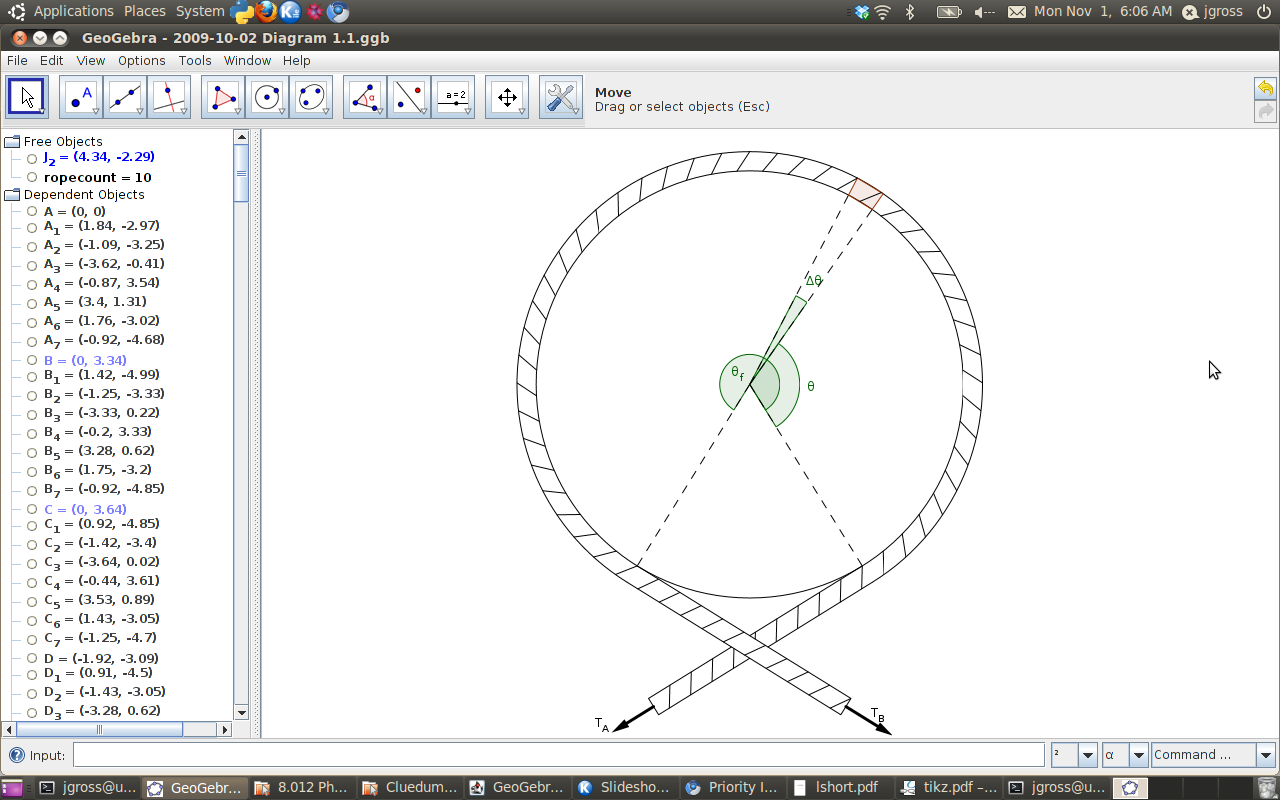
\includegraphics[width=\textwidth]{geogebra1} \\
      \end{center}
    \end{frame}
    \begin{frame}
      \frametitle{Geogebra}
      \begin{center}
        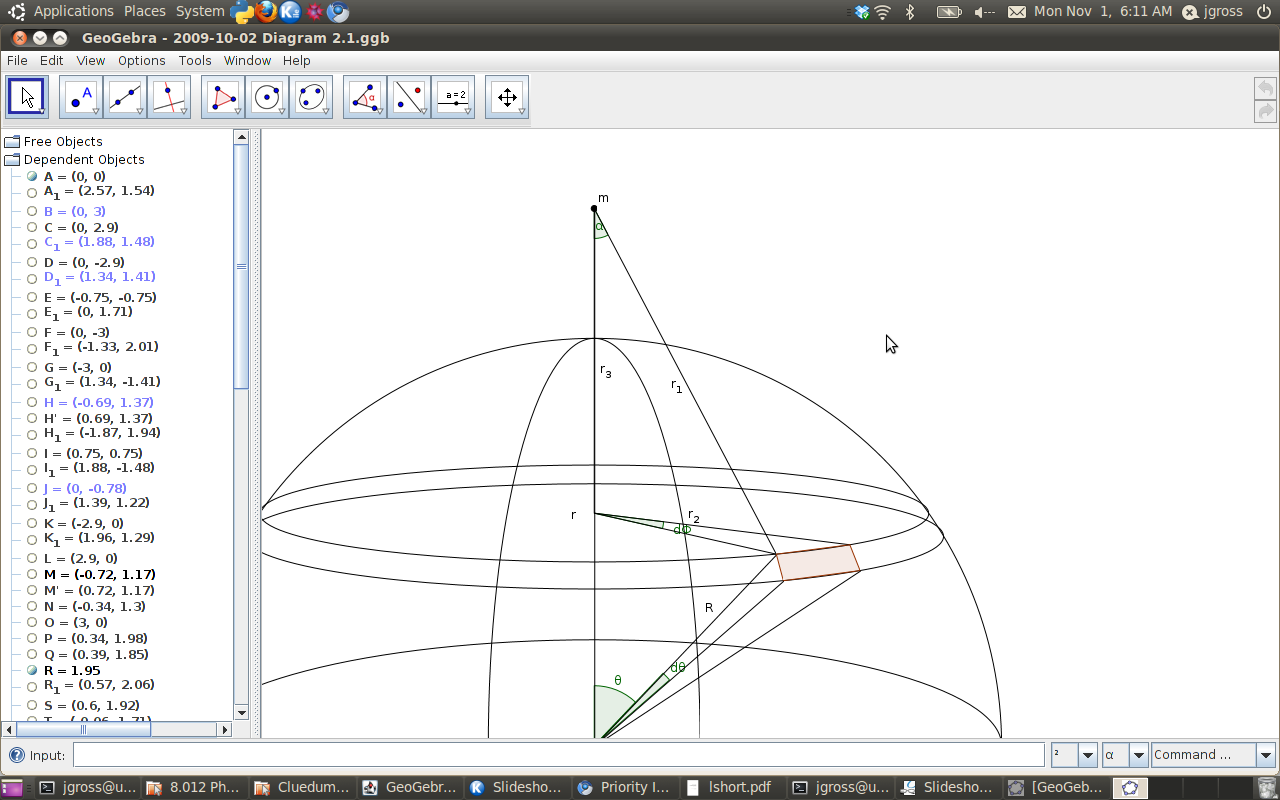
\includegraphics[width=\textwidth]{geogebra2} \\
      \end{center}
    \end{frame}
    \begin{frame}
      \frametitle{Geogebra}
      \begin{center}
        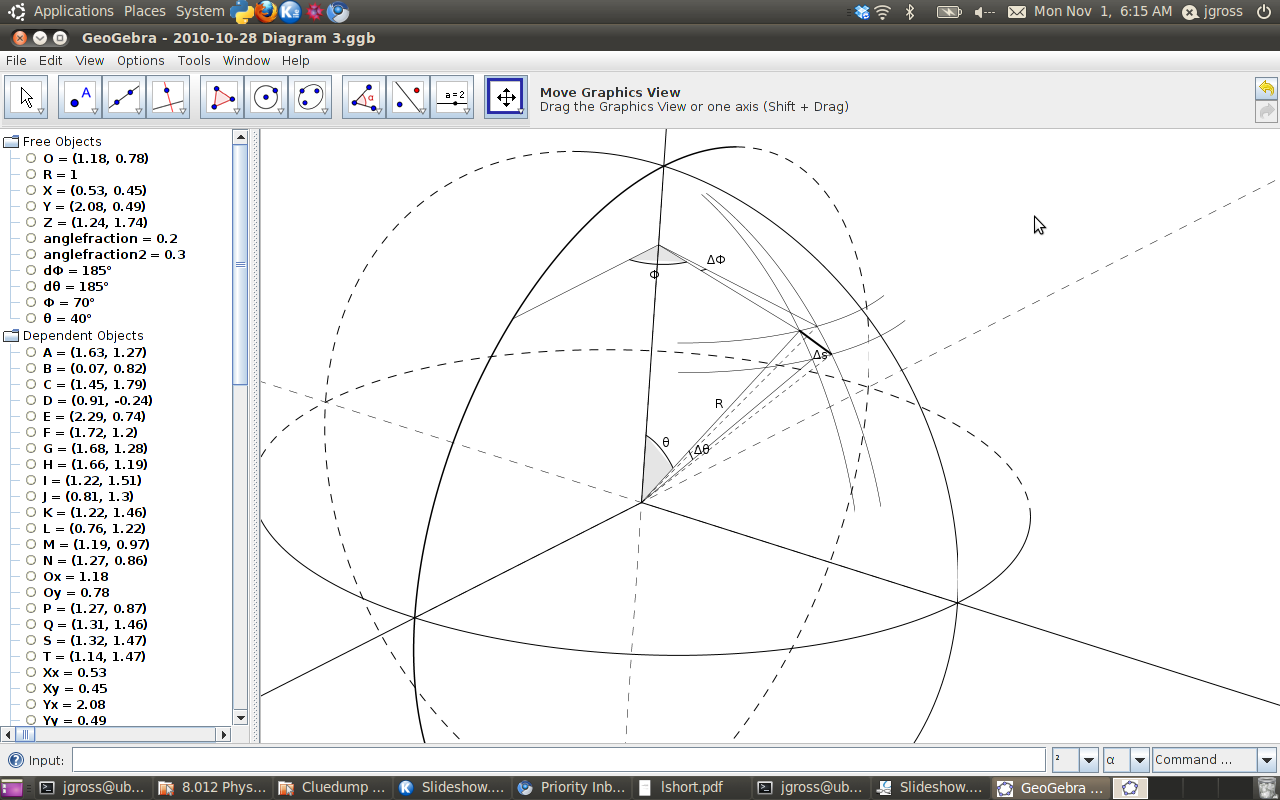
\includegraphics[width=\textwidth]{geogebra3} \\
      \end{center}
    \end{frame}
    \begin{frame}
      \frametitle{Geogebra}
      \begin{itemize}
        \item Exports to pgf/tikz, pdf, png, and others.
        \item Great for geometrical figures.
        \item Allows labeling with (almost) arbitrary LaTeX formulas.
        \item Sometimes requires a bit of manual tweaking.
      \end{itemize}
    \end{frame}
    \begin{frame}
      \frametitle{Inkscape + inkscape2tikz + TeXText}
      \begin{itemize}
        \item Great for arbitrary vector graphics.
        \item Good when you want to draw a diagram by hand.
        \item Doesn't seem to support exporting text as tikz, though TeXText lets you insert LaTeX for export as pdf.
      \end{itemize}
    \end{frame}
    \begin{frame}
      \frametitle{Asymptote}
      \begin{itemize}
        \item Standard for \LaTeX{} diagrams
        \item Extraordinarily powerful
        \item Requires an extra program to \TeX{} your documents
      \end{itemize}
      \begin{center}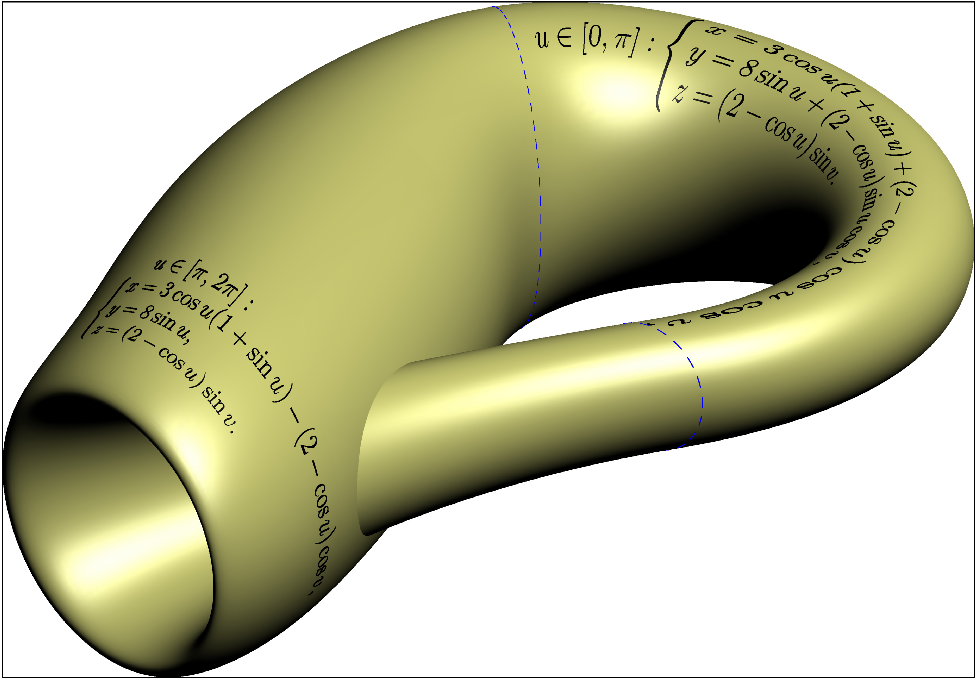
\includegraphics[width=0.5\textwidth]{Klein}\end{center}
    \end{frame}
    \begin{frame}
      \frametitle{xfig}
      \begin{itemize}
        \item Good for very large files
        \item Old and not very good interface
        \item Steep learning curve
      \end{itemize}
      \begin{center}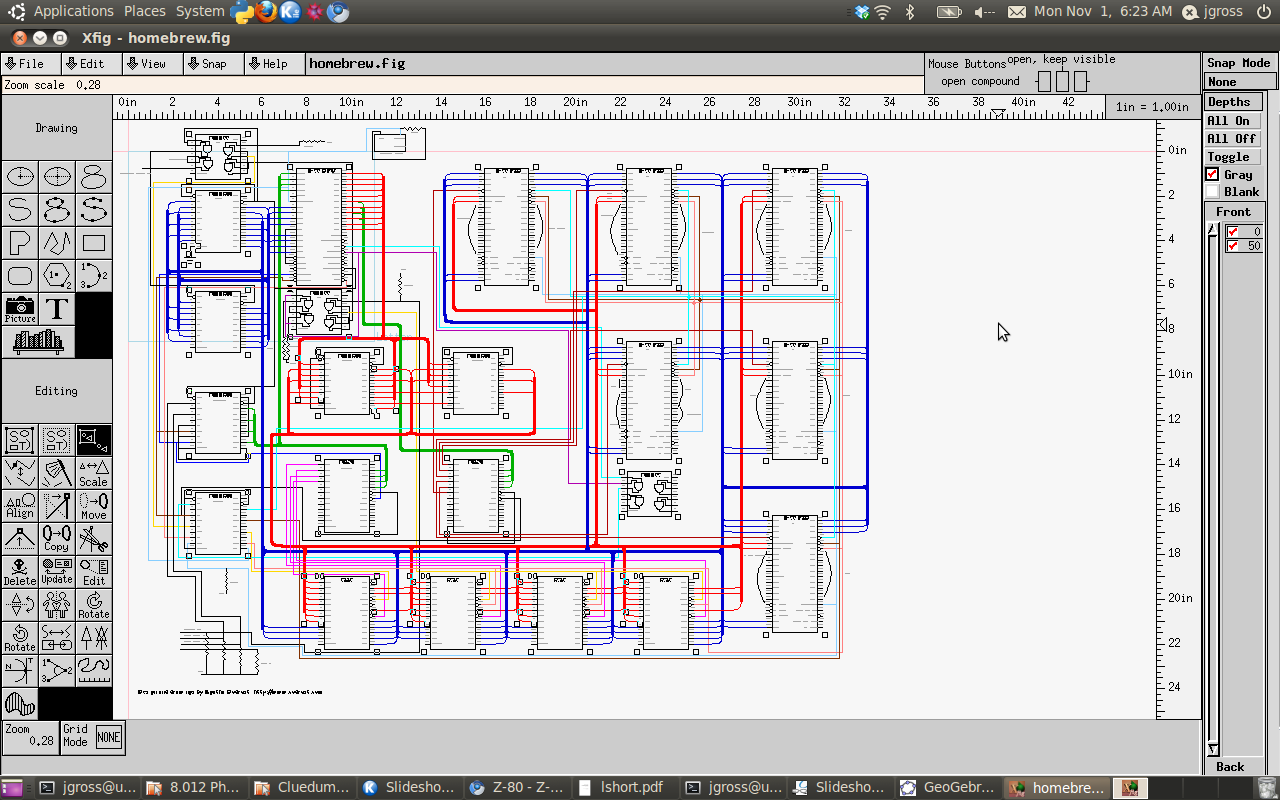
\includegraphics[width=0.5\textwidth]{xfig}\end{center}
    \end{frame}
\section*{}
    \begin{frame}
      \frametitle{Exercises}
      \begin{itemize}
        \item Should take you 2--20 hours
        \item Email me if you want help
        \item Can be found at \url{http://web.mit.edu/jgross/Public/2010cluedump/exercises.pdf}
      \end{itemize}
    \end{frame}
    \begin{frame}
      \frametitle{Thank You}
      \fontsize{128}{0}\selectfont\begin{center}Thank You!\end{center}
    \end{frame}
\end{document}
